\newpage
\section{Model To Tree with TGGs}

This is the second half of our round trip. You may have noticed after running \emph{TGGMain} in the forward direction, that the backwards transformation also
succeeded. This transformation used the \texttt{tree.xmi\_fwd.xmi} model (generated from your original text) and drove it through another transformation to
change it \emph{back} to a tree, where it will be transformed one more time by the ANTLR unparser to get back to our original text format.

Lets compare this resulting file, \texttt{tree.xmi\_FWD.xmi\_BWD.xmi}, against our original \texttt{tree.xmi} model.

%\usepackage{graphics} is needed for \includegraphics
\begin{figure}[htp]
\begin{center}
  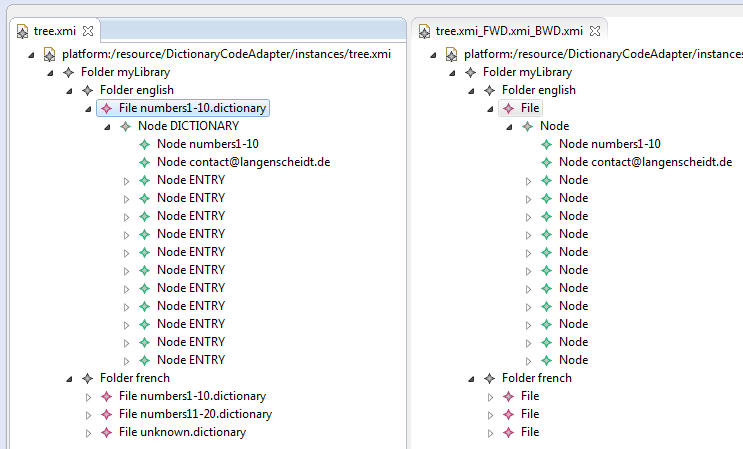
\includegraphics[width=\textwidth]{eclipse_generatedBackwardsModel}
  \caption[labelInTOC]{needs refinement\ldots}
  \label{eclipse:generatedBkwrdMdl}
\end{center}
\end{figure}

You can see that some things need to be fixed up -- we're missing the ``DICTIONARY'' and ``ENTRY" headings of the major nodes. Obviously, some refinement is
needed here..

Note:: oarser requires that all attribute constraints are declared before link variables.


\begin{figure}[htp]
\begin{center}
  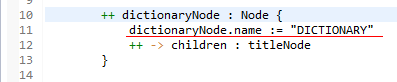
\includegraphics[width=\textwidth]{eclipse_NodeToDictionaryRule_updated}
  \caption[labelInTOC]{needs refinement\ldots}
  \label{eclipse:generatedBkwrdMdl}
\end{center}
\end{figure}

\begin{figure}[htp]
\begin{center}
  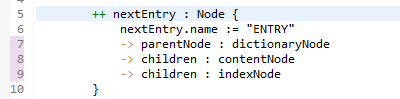
\includegraphics[width=\textwidth]{eclipse_ForAllEntryRule_updated}
  \caption[labelInTOC]{needs refinement\ldots}
  \label{eclipse:generatedBkwrdMdl}
\end{center}
\end{figure}
\newpage
\hypertarget{m2tvis}{}
\subsection{Double-checking the TGG}
\visHeader

\begin{itemize}

\item[$\blacktriangleright$] Open \texttt{NodeToDictionaryRule} and update as depicted below (via attribute constraint). Is this in the right place? Should this
be done before??

\begin{figure}[htp]
\begin{center}
  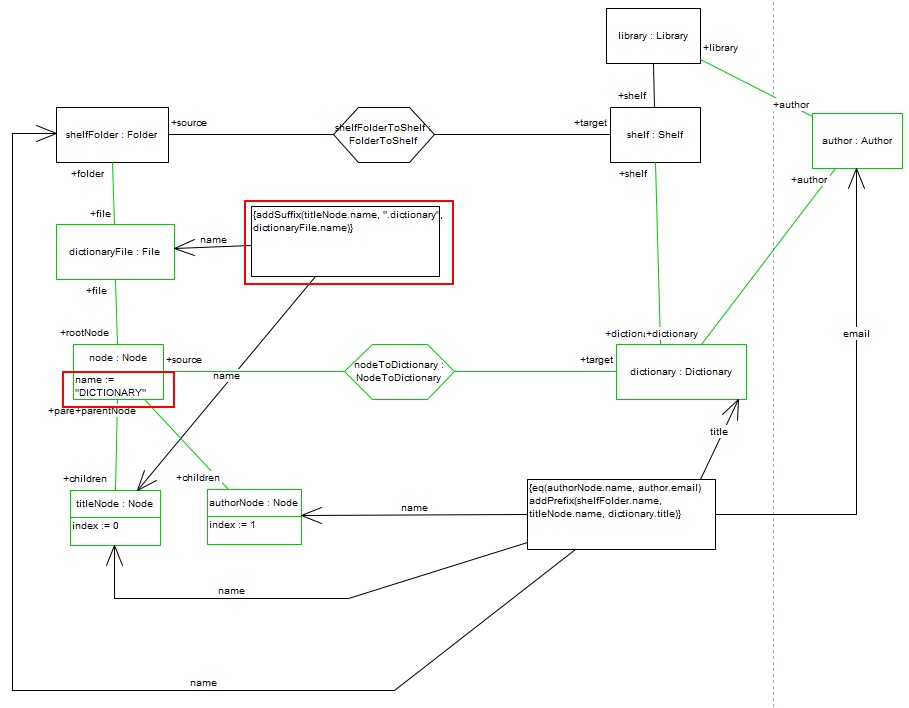
\includegraphics[width=\textwidth]{ea_updateNodeToDictionary}
  \caption{updated NodeToDictionary}
  \label{ea:NodeToDictionary_updated}
\end{center}
\end{figure}

\item[$\blacktriangleright$] Similarly, open \texttt{ForAllEntry} in EA and update like so:

\begin{figure}[htp]
\begin{center}
  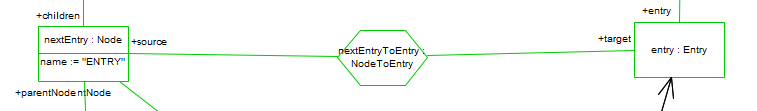
\includegraphics[width=\textwidth]{ea_updateForAllEntry}
  \caption{updated ForAllEntry}
  \label{ea:ForAllEntry_updated}
\end{center}
\end{figure}

\item[$\blacktriangleright$] End comment.

\jumpSingle{finalStep}

\end{itemize}


\newpage
\hypertarget{m2ttex}{}
\subsection{Refining the TGG Transformation}
\texHeader

\begin{itemize}

\item[$\blacktriangleright$] Find the relevant files and add the following attribute constraints. Note : the MOSL parser requires that all attribute constraints
are declared before link variables.

\begin{figure}[htp]
\begin{center}
  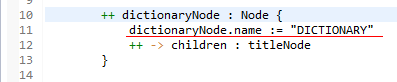
\includegraphics[width=0.8\textwidth]{eclipse_NodeToDictionaryRule_updated}
  \caption[labelInTOC]{needs refinement\ldots}
  \label{eclipse:generatedBkwrdMdl}
\end{center}
\end{figure}

\begin{figure}[htp]
\begin{center}
  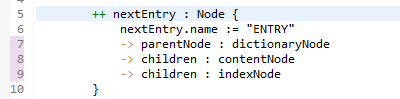
\includegraphics[width=0.8\textwidth]{eclipse_ForAllEntryRule_updated}
  \caption[labelInTOC]{needs refinement\ldots}
  \label{eclipse:generatedBkwrdMdl}
\end{center}
\end{figure} 

\item[$\blacktriangleright$] Add new SetDefaultNumber CSP here.

\begin{figure}[htbp]
\begin{center}
  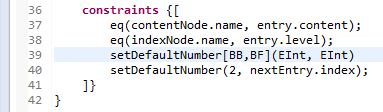
\includegraphics[width=0.6\textwidth]{eclipse_setDefaultNumberConstraint}
  \caption{extra constraint}
  \label{eclipse:newEntryConstraint}
\end{center}
\end{figure}

\end{itemize}

